%max: 5pages

\documentclass{llncs}
%
\usepackage{makeidx}  % allows for indexgeneration
\usepackage{graphicx} % for photos
%
\begin{document}
%
\frontmatter          % for the preliminaries
%
\pagestyle{headings}  % switches on printing of running heads
\addtocmark{Hamiltonian Mechanics} % additional mark in the TOC
%

\mainmatter              % start of the contributions
%
\title{Zone-project: towards a better news feed using semantic web}
%
\titlerunning{Zone-project}  % abbreviated title (for running head)
%                                     also used for the TOC unless
%                                     \toctitle is used
%
\author{Christophe Desclaux\inst{1}}
%
\authorrunning{Christophe Desclaux} % abbreviated author list (for running head)
%
%%%% list of authors for the TOC (use if author list has to be modified)
\tocauthor{Christophe Desclaux}
%
\institute{Wimmics Inria, Sophia Antipolis...,\\
\email{christophe@zouig.org},\\ WWW home page:
\texttt{http://www.zone-project.org}
}

\maketitle

\begin{abstract}%
Nowadays we can use RSS feeds, Twitter, Google Reader, Yahoo Pipes or aggregators to keep up with news. Though those solutions do not guarantee data privacy and rather manage news by origin. The zone project proposes an innovative solution to overcome those issues using the power of Semantic Web and group related informations together.
ZONE-project provides a new, innovative way to follow news. At its core, the system is aggregating news items from various RSS feeds.
Using the power of semantic web we are able to efficiently tag and annotate each news. Those tags are the basis of filters.
Filters allow users to see only news that are relevant. For instance users can retrieve all news containing a tag, or on the contrary never see news containing specific tags.


%The abstract should summarize the contents of the paper
%using at least 70 and at most 150 words. It will be set in 9-point
%font size and be inset 1.0 cm from the right and left margins.
%There will be two blank lines before and after the Abstract. \dots
\keywords{linked data, data aggregation, RSS}
\end{abstract}
%
\section{Motivation}
%
A lot of news are published every day on internet, the number of news websites has increased significantly. People and organization are now building news aggregators in order to sort all this information. This systems are really important in order to clean all the amount of information.

Solutions exists, you can for example use \textsl{Google news} \footnote{\url{http://news.google.fr}} like a trusted provider of information, but in this web application your are only a consumer and don't have a lot of interaction with the system. 

The second solution is to make news forecasting using \textsl{Twitter}\footnote{\url{http://www.twitter.com}}, it's a  solution in which you have the hand on your sources. You can clearly choose the users you want to follow. But you can't have a selection on sources and on topics and you have a lot of noise around goods informations.

The last revelant solution that you can use is \textsl{Yahoo Pipes} \footnote{\url{http://pipes.yahoo.com/pipes/}}, this tool allows the mixing of popular data feeds to create data filtering via a visual editor. It ue pipes as workflows which will help users to sort feeds.

With the study of this three solutions I have extract some main challenges that good aggregators need to work on.
\begin{itemize}
  \item \textbf{filtering capacities} he need to sort all information according to [critères fins]
  \item \textbf{lot of informations} the tool need to have access to all news present on internet 
  \item \textbf{privacy} users need to use the solution independently of any source provider.
\end{itemize}

Technicals solutions exists in order to solve this challenges, Google solve this problem using [article de Larry Page sur l'aggregation par mots clés] but this solution is not much efficient because it work on words instead of working on meaning. The solution to use is to use aggregation based on semantic web. 

We will first present in this article how work our solution called Zone with explications about the annotation workflow, the ontologie used and the use of datamining solutions. The we will present a demonstration of the application and finally conclude and talk about future work.

%
\section{Application: Zone}


\subsection{the workflow}
%
In order to have a selection more efficient of news according to their semantic relevance, we have create two sort of workflows, according to the following figure \ref{fig:WF} which show the general architecture: a semantic annotation workflow of news and a filtering workflow. The distinction between the two workflows is [very very] important in order to work [de manère asynchrone].


\begin{figure}[htb!]
	\begin{centering}
	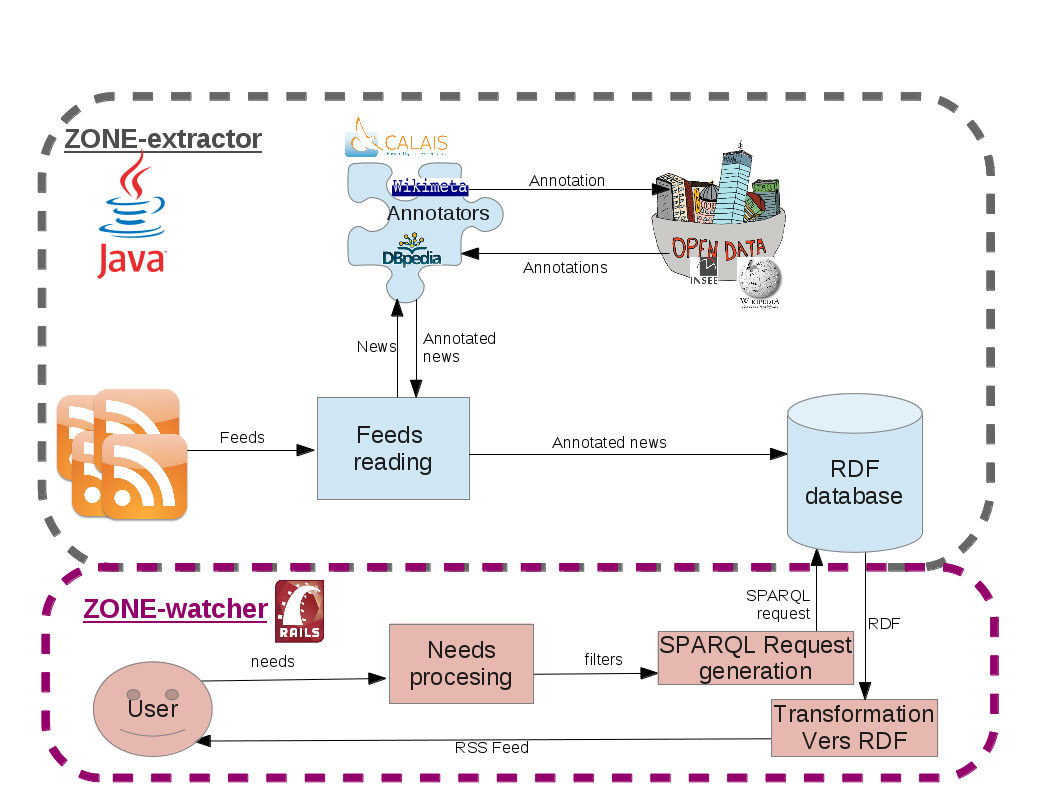
\includegraphics[width=1\textwidth]{diagramArchi.png}
	\caption{Workflows d'annotation et de filtrage sémantique de nouvelles}
	\label{fig:WF}
	\end{centering}
\end{figure}

\subsubsection{The semantic annotation workflow}
The annotation workflow crawled the web extracting all news and storing them in database next to semantic annotations.
In order to make the news retreival we use RSS feeds technologies and will not present them in details. The storage of the news is made 
We will present more in details the annotation procesus and the use of links with linkedOpenDatas, for the news retreival we ue techno

\subsubsection{The filtering workflow}

%
\subsection{The ontologie}
%
basée sur RSS
on a ajouté un schéma RDFs spécialisé
on se base aussi sur l'ontologie de wikimeta/insee
%

%
\subsection{Using datamining}
section d'Ameni

\section{Demonstration}
%
On va sur l'application, on séléctionne les entitées nommées qui nous interessent dans la liste des articles présents, ca génère ce qu'on a envie de voir...
Comment se déroule la démo, captures
%

\section{Conclusion and futur work}
%
Challenges qui restent à résoudre :
	*tech : faire des liens vers openData et du raisoning
	*com : trouver moyen de pérenniser le projet
%

\section{Acknowledgments}
%
Description du contexte de travail=> se passe à l'inria BYC... équipe wimmics qui bosse sur semantic web

%





%
% ---- Bibliography ----
%
\begin{thebibliography}{5}
%
\bibitem {clar:eke}
Clarke, F., Ekeland, I.:
Nonlinear oscillations and
boundary-value problems for Hamiltonian systems.
Arch. Rat. Mech. Anal. 78, 315--333 (1982)

\bibitem {clar:eke:2}
Clarke, F., Ekeland, I.:
Solutions p\'{e}riodiques, du
p\'{e}riode donn\'{e}e, des \'{e}quations hamiltoniennes.
Note CRAS Paris 287, 1013--1015 (1978)

\bibitem {mich:tar}
Michalek, R., Tarantello, G.:
Subharmonic solutions with prescribed minimal
period for nonautonomous Hamiltonian systems.
J. Diff. Eq. 72, 28--55 (1988)

\bibitem {tar}
Tarantello, G.:
Subharmonic solutions for Hamiltonian
systems via a $\bbbz_{p}$ pseudoindex theory.
Annali di Matematica Pura (to appear)

\bibitem {rab}
Rabinowitz, P.:
On subharmonic solutions of a Hamiltonian system.
Comm. Pure Appl. Math. 33, 609--633 (1980)

\end{thebibliography}

\clearpage
\end{document}